\chapter{Introducción}
\label{cap:introduccion}
En este capítulo se ubicará el proyecto en el contexto de la robótica móvil y se enumeraran los distintos problemas que se presentan en este contexto. En el siguiente aparatado hablaremos de la creación de mapas y sus utilidades. También se expondrá qué es la RoboCup@Home, ya que es una parte importante en este proyecto por ser el escenario de numerosas pruebas llevadas a cabo. Por último se expondrá la estructura de la memoria y se explicarán brevemente las partes por las que está formada.

\section{Robótica móvil}
\label{cap:roboticamovil}
Los robots móviles son máquinas con la capacidad de desplazarse por un entorno. Para ello hacen uso de un sistema de automoción, ya sean ruedas, patas u orugas. 
La robótica móvil está sufriendo un gran crecimiento debido al abaratamiento del hardware y las grandes oportunidades que nos ofrecen, tanto en materia de educación como en materia industrial. 
Cuando nos encontramos con un problema en el que un robot móvil puede ser la mejor solución tendremos que tener en cuenta los siguientes problemas a solucionar:
\begin{itemize}
\item \textbf{Percepción} Para resolver este problema equiparemos a nuestro robot de sensores, como puede ser una cámara, un láser, sensores de odometría o bumpers para obtener información acerca de qué hay en el escenario en el que se encuentra el robot.
\item \textbf{Localización} Una vez resuelto el problema de conocer que hay cerca del robot, necesitamos conocer la posición del robot dentro del escenario. Esto se puede resolver con algoritmos como MonteCarlo, con cámaras cenitales, triangulación con balizas, etc. Para resolver la localización también es común el uso de mapas. 
\item \textbf{Navegación} La característica principal de los robots móviles es que tienen la capacidad de desplazarse, pero la navegación no solo se cumple cuando el robot se mueve, el robot debe moverse a un punto determinado, de una forma segura, es decir sin chocar con los objetos del escenario, y de la forma más eficaz posible. Dentro de la navegación se pueden distinguir 2 partes, la navegación local que se ocupa del movimiento del robot y de evitar obstáculos y la navegación global qué establece rutas.
\item \textbf{Inteligencia} El siguiente problema se encuentra en un nivel de abstracción más alto. El problema de la inteligencia se refiere a qué tiene que hacer el robot, qué finalidad debe cumplir.
\item \textbf{Autonomía} Habrá momentos en los que el robot deberá tomar algunas decisiones, en referencia a su estado en el escenario, por ejemplo si se acerca mucho a una pared, o si llega a su destino correctamente.
\item \textbf{Interacción con los humanos} Los robots suelen crearse para facilitarnos una tarea o asistirnos en nuestro día a día, por esto los robots deben contar con una interfaz hombre-maquina con la que comunicarnos cosas o con la que nosotros podamos ayudar al robot para así mejorar sus acciones.
\end{itemize}

\section{Mapeado}
\label{cap:mapeado}
Crear un mapa de un escenario puede sernos realmente útil ya que servirán al robot como fuente de información para resolver problemas de Localización y de Navegación. Estos mapas pueden ser creados por un humano, midiendo las paredes y los objetos de un escenario para más tarde transformarlo en una imagen que el robot pueda leer, o puede ser creado directamente con un robot móvil. Esta segunda opción nos permite realizar mapas de zonas que pueden resultar inaccesibles para el ser humano, como puede ser una zona radioactiva u otro planeta del sistema solar.

\begin{figure}[hbtp]
  \begin{center}
    \subfigure[Mapa láser]{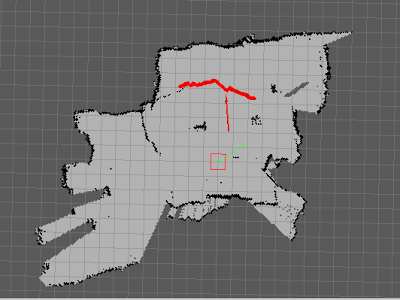
\includegraphics[width=6cm,height=5cm]{img/cap1/mapa1}}
    \subfigure[Mapa RGBD]{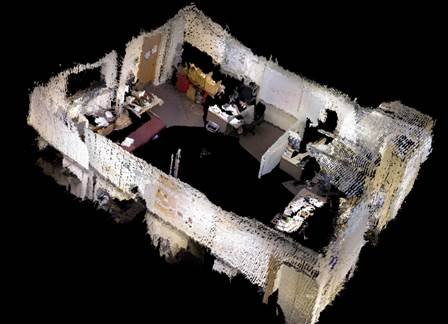
\includegraphics[width=6cm,height=5cm]{img/cap1/mapa2}}
  \end{center}
  \caption{Ejemplos de mapas}
  \label{fig:maps-ej}
\end{figure}
Para llevar a cabo el mapeo de un escenario con un robot móvil deberemos equipar a nuestro robot con sensores capaces de medir distancias, tales como una cámara RGBD o un láser. La cámara RGBD nos proporciona una nube de puntos en 3D, por lo que nos proporciona una información muy rica del entorno pero el tratamiento de esta información resulta muy costoso. El láser nos proporciona un array de distancias en 270º, estas distancias suelen ser muy precisas y su tratamiento es muy liviano, aunque solo contamos con el plano en el que se ubica el láser. 

En ese trabajo se expondrá una nueva opción de mapeado que resultará de la mezcla de las dos opciones vistas anteriormente. Partiremos de un mapa creado por nosotros de un escenario y el robot irá añadiendo dinámicamente los objetos que vaya encontrando y no estén representados en este mapa inicial. Esta nueva visión nos ha proporcionado muy buenos resultados, tanto que fue integrada como algoritmo de navegación en el robot del equipo GentleBots, del cual formamos parte, y con el que participamos en la Robocup 2016 de Leipzig, en la categoría RoboCup@Home.



\section{RoboCup y RoboCup@Home}
\label{cap:robocup}
La RoboCup\footnote{http://www.robocup.org} es un proyecto internacional que se constituyó en 1997 y que tiene por objetivo el promover la investigación y educación sobre inteligencia artificial. La misión por la que se constituyó esta iniciativa fue la de crear un equipo de robots completamente autónomos que fueran capaces de ganar a la selección de fútbol ganadora de la Copa del Mundo en el año 2050. Desde sus inicios, esta competición ha experimentado una gran expansión y ahora abarca disciplinas tales como: Robótica doméstica, industrial, de rescate, competiciones infantiles, etc.

Las competencias más destacadas que abarca la competición son, aunque dentro de cada una puede haber distintas ligas:
\begin{itemize}
  \item \textbf{RoboCupSoccer:} Categoría de fútbol con robots móviles autónomos. La diferencia entre las ligas reside en la morfología de los robots ya que existen ligas para pequeños y gran robots con ruedas, para robots humanoides y para robots simulados.
\begin{figure}[H]
  \begin{center}
    \subfigure[Robocup soccer robot movil]{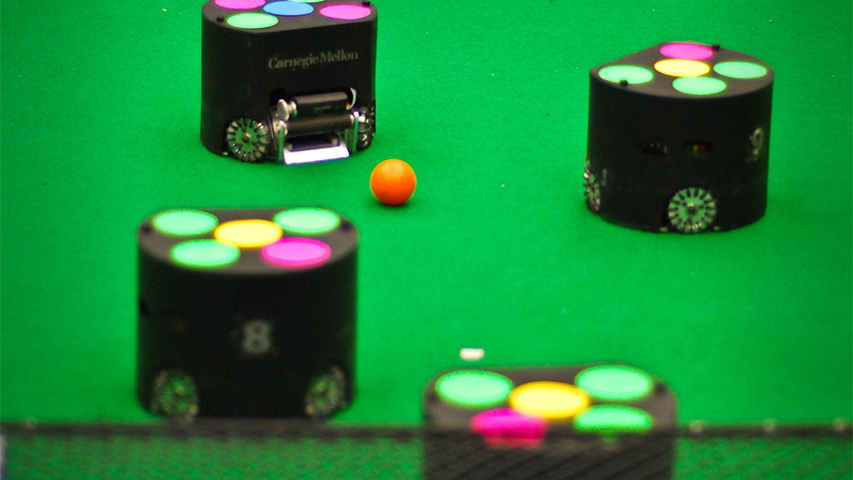
\includegraphics[width=6cm,height=5cm]{img/cap1/robocup-soccer}}
    \subfigure[Robocup soccer nao]{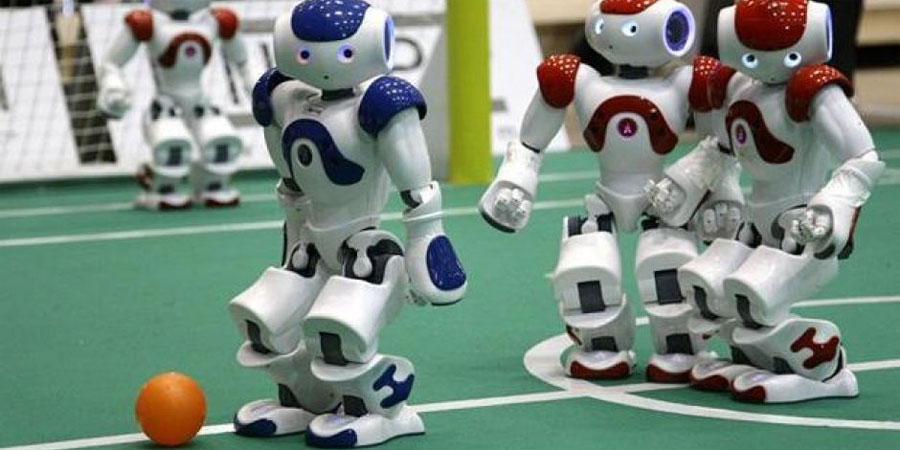
\includegraphics[width=6cm,height=5cm]{img/cap1/robocup-nao}}
  \end{center}
  \caption{Robocup Soccer}
  \label{fig:maps-ej}
\end{figure}
  \item \textbf{RoboCupRescue:} Categoría de robots autónomos o teleoperados capaces de desplazarse, operar y rescatar víctimas en escenarios que simulan un terreno desfavorable, como puede ser el que se puede encontrar tras un desastre natural o en un conflicto bélico.
  \begin{figure}[H]  
  \begin{center}
    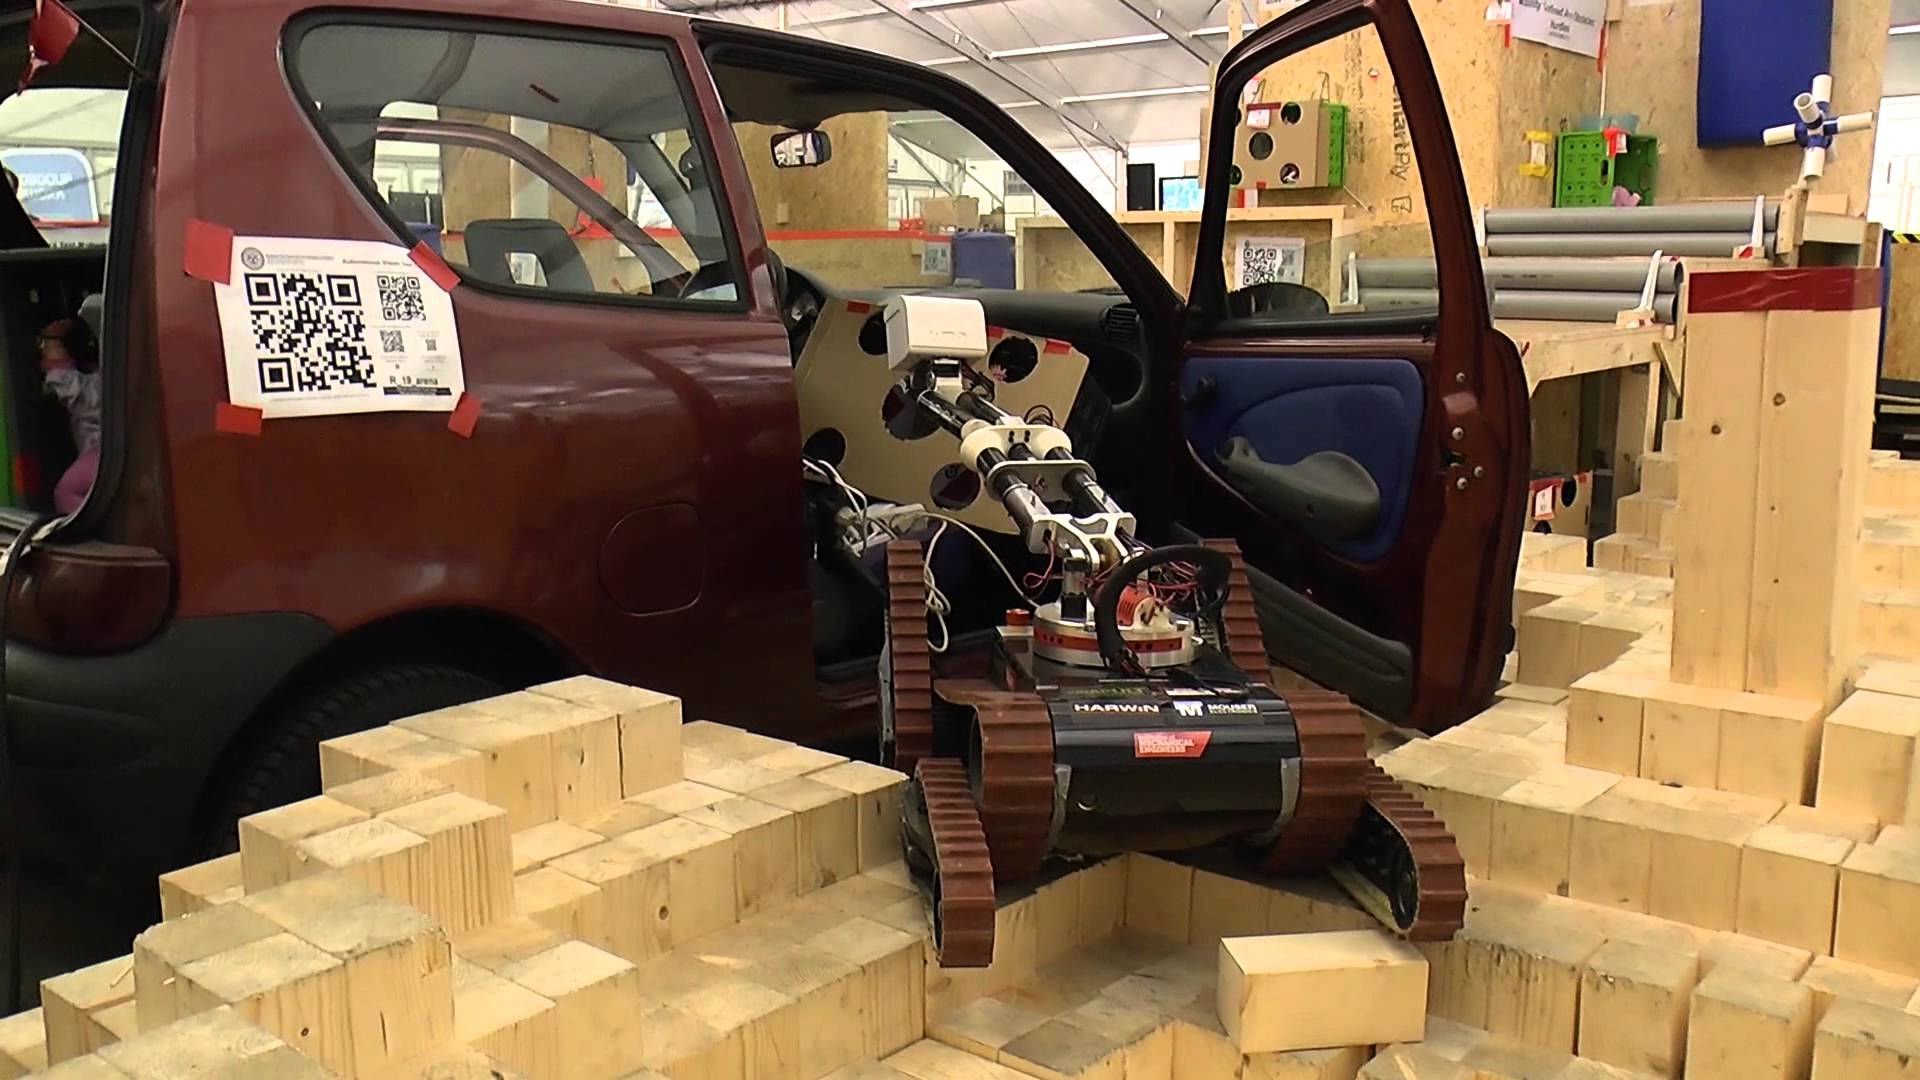
\includegraphics[width=7cm,height=5cm]{img/cap1/robocup-rescue}
  \end{center}
  \caption{Robocup Rescue.}
  \label{fig:robocup-rescue}
\end{figure}
  \item \textbf{RoboCupJunior:} Categoría orientada a acercar la competición a estudiantes de primaria y secundaria. Dentro de esta categoría existen ligas adaptadas de fútbol y rescate y una categoría de baile.
  \begin{figure}[H]  
  \begin{center}
    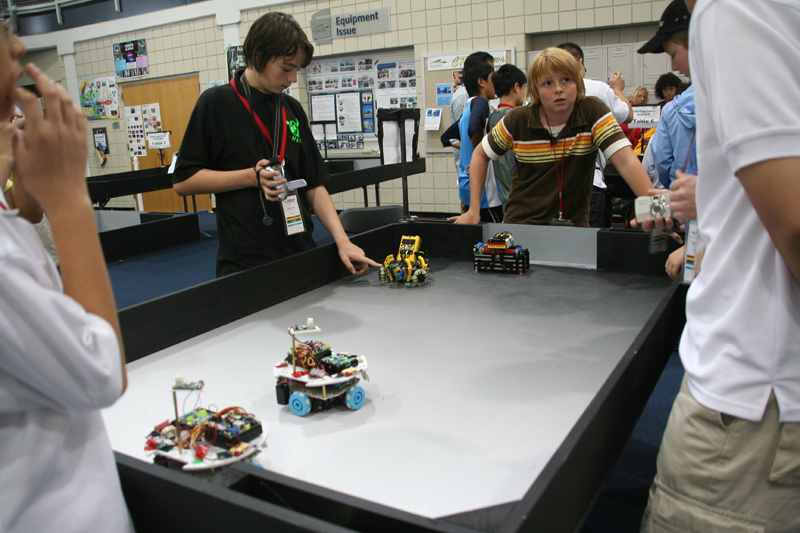
\includegraphics[width=7cm,height=5cm]{img/cap1/robocup-junior}
  \end{center}
  \caption{Robocup Junior.}
  \label{fig:robocup-junior}
\end{figure}
  \item \textbf{RoboCup@Home:} Categoría que tiene como objetivo desarrollar la tecnología de robots de servicio y asistencia para futuras aplicaciones domésticas.
  \begin{figure}[H]  
  \begin{center}
    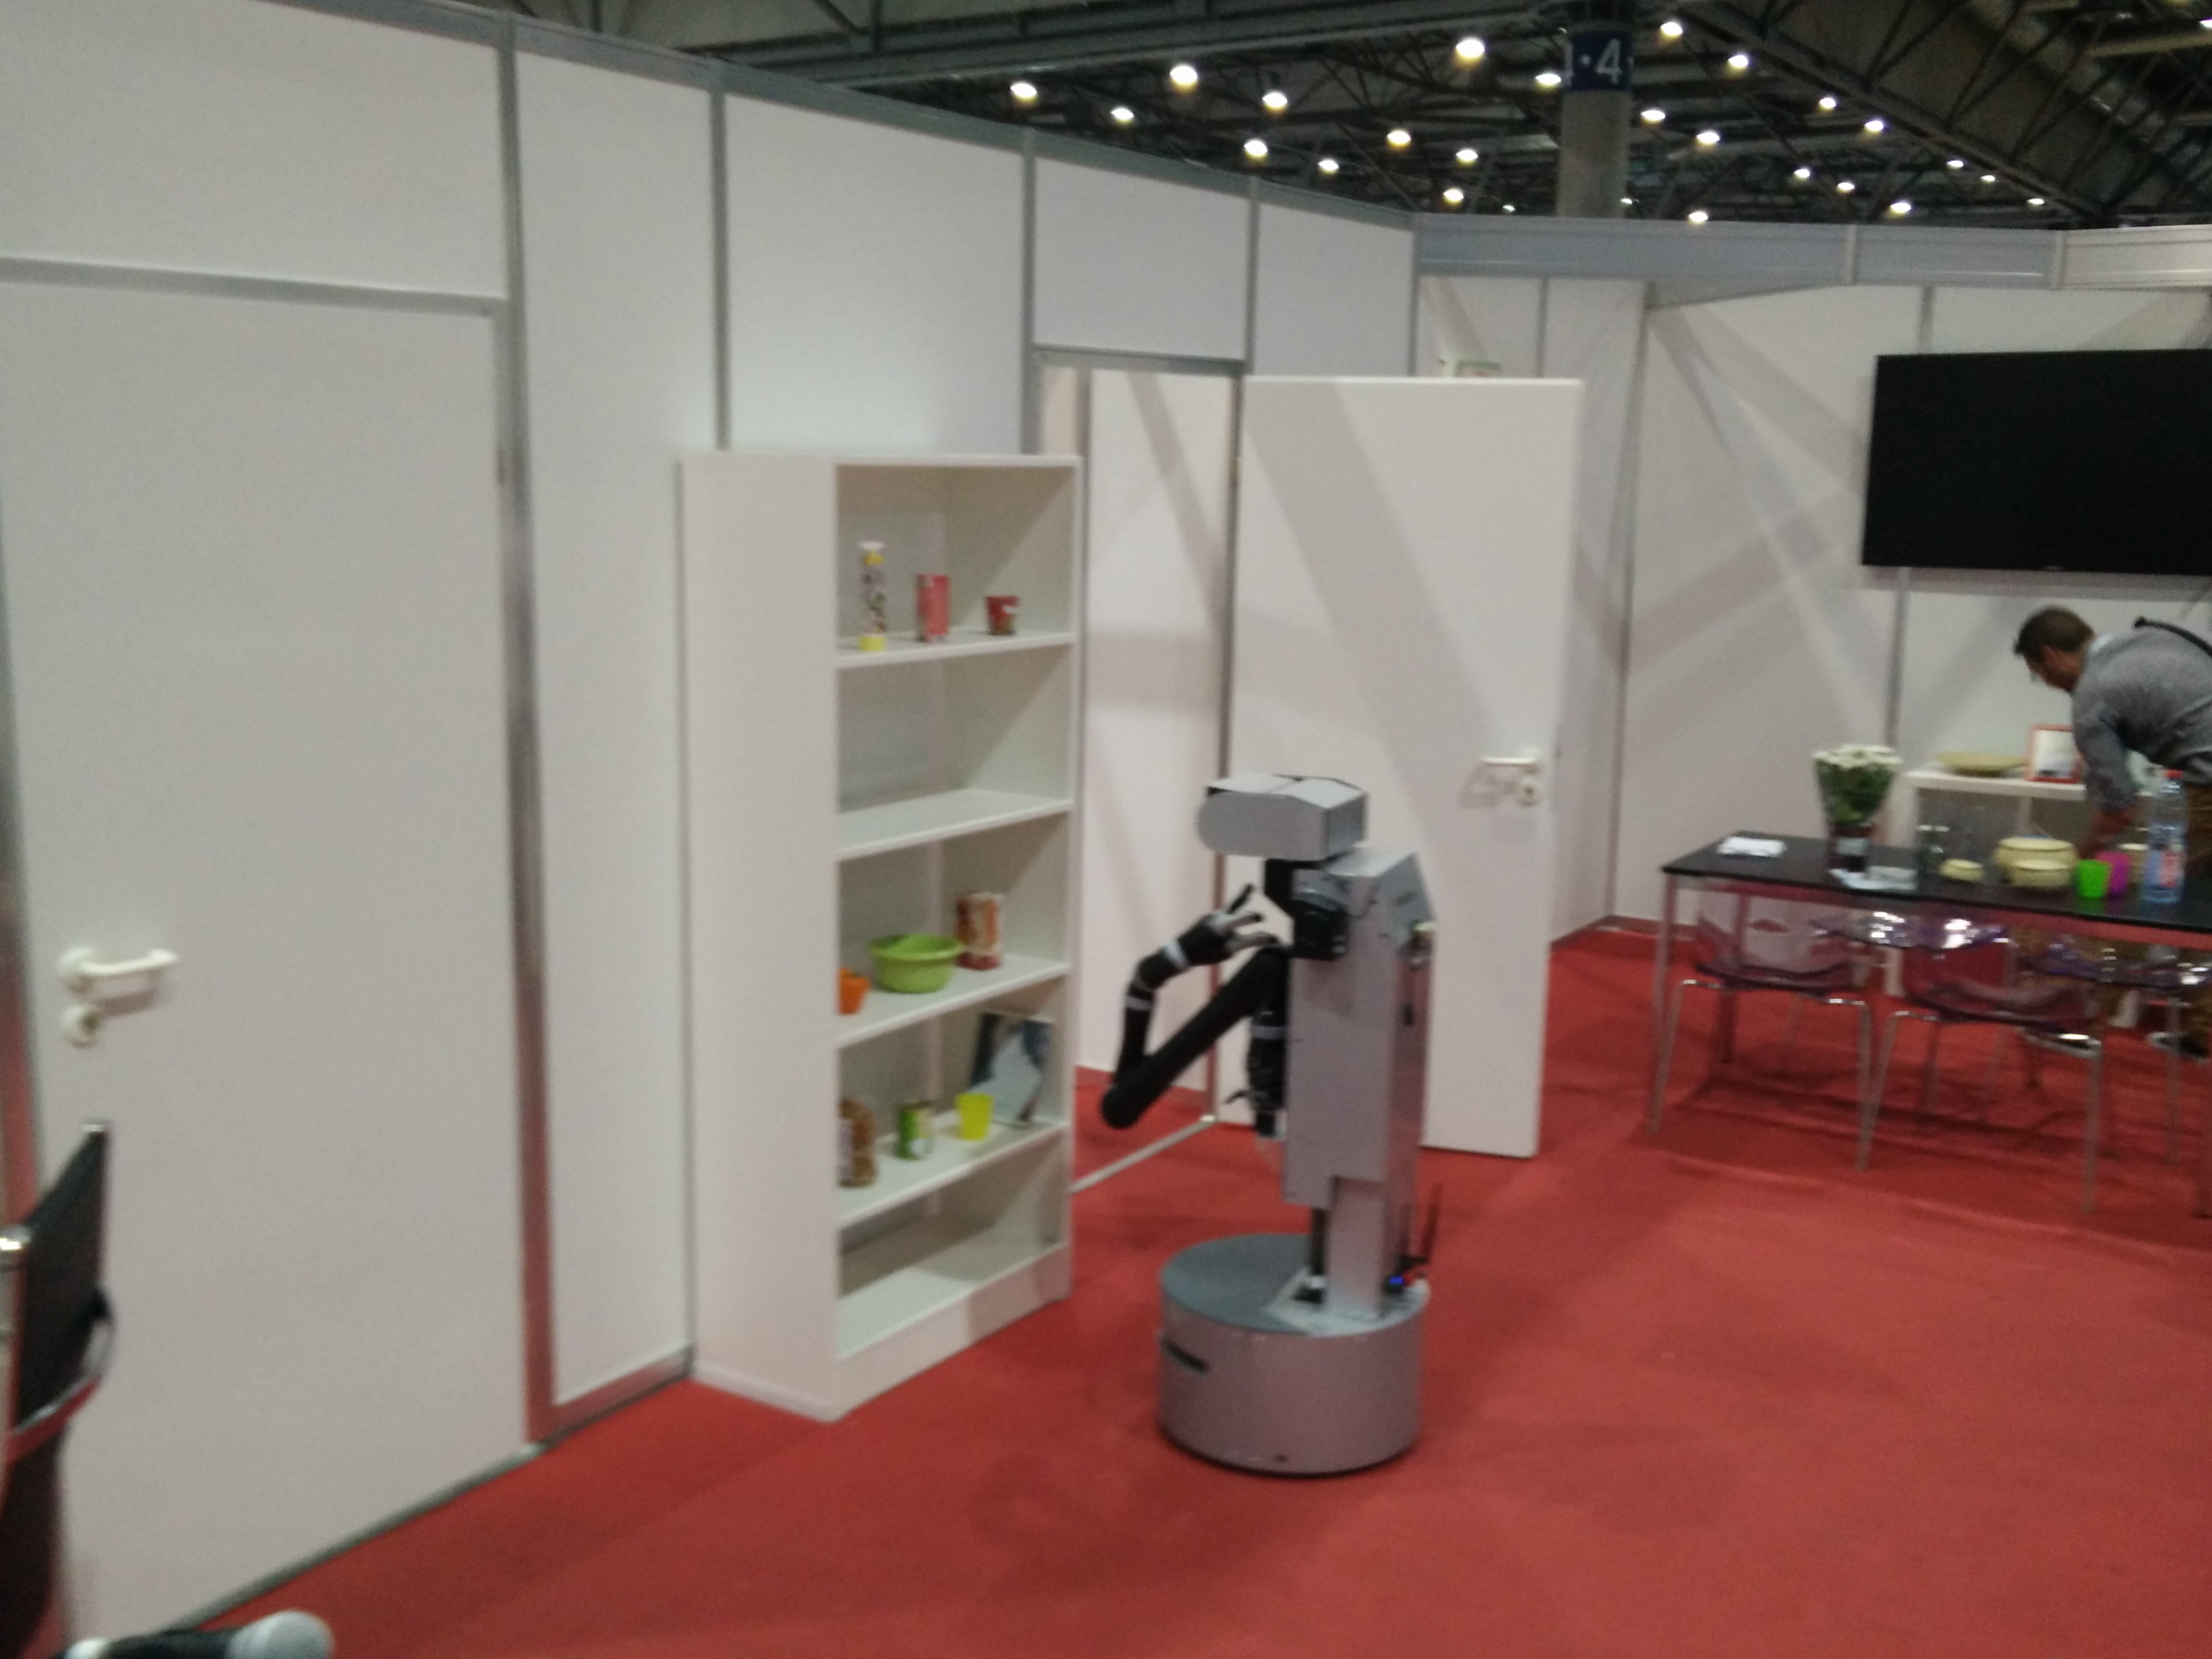
\includegraphics[width=7cm,height=5cm]{img/cap1/robocup-home}
  \end{center}
  \caption{Robocup Home.}
  \label{fig:robocup-home}
\end{figure}
\end{itemize}

Profundizaremos un poco más en la categoría Home.

\subsection{RoboCup@Home}
\label{cap:robocuphome}
Como se ha expuesto anteriormente esta categoría se centra en el desarrollo y la aplicación de robots autónomos móviles al ámbito doméstico.
\begin{figure}[hbtp]  
  \begin{center}
    
\includegraphics[width=5cm]{img/cap1/logoRobocupHome}
  \end{center}
  \caption{Robocup@Home.}
  \label{fig:logoRobocupHome}
\end{figure}

Se utiliza un conjunto de pruebas de referencia  para evaluar las capacidades y el rendimiento de los robots en un entorno del hogar no estandarizado. La atención se centra en los siguientes dominios, pero no se limita exclusivamente a ellos:

\begin{itemize}
\item \textbf{Interacción y cooperación robot-humano} 
\item \textbf{Navegación y cartografía en entornos dinámicos} 
\item \textbf{Visión artificial y reconocimiento de objetos en condiciones de luz natural} 
\item \textbf{Manipulación de objetos} 
\item \textbf{Comportamientos adaptativos} 
\item \textbf{Integración de comportamientos}
\item \textbf{Inteligencia ambiental}  
\item \textbf{Normalización e integración de Sistemas}  
\end{itemize}


Las principales pruebas que se usan para evaluar las competencias antes descritas son:
\begin{itemize}
  \item \textbf{Navegación:} En esta prueba se evalúa la capacidad de navegar por dentro de un escenario doméstico sin chocar con nada y pudiendo sortear objetos grandes, pequeños y personas que puedan obstaculizar su camino. Se propone, por parte de la organización, una serie de puntos que el robot debe alcanzar, incluso si se encontrara una puerta cerrada o un objeto que le hace imposible alcanzar su objetivo, debe tomar un camino alternativo.
  \item \textbf{Reconocimiento del habla:} En esta prueba se hace al robot una serie de preguntas pactadas, y el robot debe dirigirse a su interlocutor y contestar correctamente a dicha pregunta.
  \item \textbf{Manipulación y reconocimiento de objetos:} Esta prueba consiste en reconocer objetos cotidianos de una estantería e intentar cogerlos con el brazo articulado que debe poseer el robot y dejar estos objetos en una balda vacía. 
  \item \textbf{Following and guiding:} Se reconocerá a un arbitro que se colocará delante del robot y se le seguirá sin perderse, saliendo desde la casa, por el recinto de la competición. Cuando el árbitro decida el robot deberá dar la vuelta y guiar al árbitro de nuevo hasta la casa.
\end{itemize}


Cada año el escenario en el que se realizan las pruebas se actualiza para parecerse cada vez más a un escenario real de un ambiente doméstico. En los primeros años solo constaba de una salón y una cocina pero cada vez se incorporan más estancias, como pasillos, habitaciones o zonas de jardín. Los escenarios del año 2016 constaban de cocina, sala de estar, habitación, pasillo y entrada. Además cada escenario tenia 3 puertas para salir al exterior.

RoboCup@Home acaba con las finales, donde los 5 equipos con las puntuaciones más altas pueden realizar la prueba final. Los equipos son calificados por un jurado formado por especialistas y no especialistas en robótica, como puede ser empresarios, especialistas en interacción hombre-máquina, personas de diseño industrial, el público o la prensa. En las finales se enfatiza menos en las cuestiones técnicas, ya que si se llega a la final significa que los equipos son muy buenos en el plano técnico.

\section{Estructura de la memoria}
\label{cap:estructuradelamemoria}
En este documento se describen los aspectos más relevantes del desarrollo del algoritmo. La memoria está dividida en ocho capítulos. En este primer capítulo se ha presentado el contexto en el que se va a desarrollar el proyecto. En el segundo capítulo se define el problema concreto y se establecen los requisitos y los objetivos del proyecto. En el tercer capítulo se exponen y describen el robot con el que se ha trabajado y las distintas herramientas que hemos utilizado o mejorado. El montaje del robot y el diseño de conectividad seguido se explica en el capítulo cuatro. En el capítulo cinco se expone el algoritmo de mapping creado. El sexto capítulo expondrá la navegación semántica desarrollada y como usa el algoritmo de mapping. En el séptimo capítulo expondremos los experimentos llevados a cabo y un pequeño diario de nuestra experiencia en la Robocup. Por último en el octavo capítulo se expondrán las conclusiones del trabajo.
